% Options for packages loaded elsewhere
\PassOptionsToPackage{unicode}{hyperref}
\PassOptionsToPackage{hyphens}{url}
\PassOptionsToPackage{dvipsnames,svgnames,x11names}{xcolor}
%
\documentclass[
  12pt,
]{article}

\usepackage{amsmath,amssymb}
\usepackage{iftex}
\ifPDFTeX
  \usepackage[T1]{fontenc}
  \usepackage[utf8]{inputenc}
  \usepackage{textcomp} % provide euro and other symbols
\else % if luatex or xetex
  \usepackage{unicode-math}
  \defaultfontfeatures{Scale=MatchLowercase}
  \defaultfontfeatures[\rmfamily]{Ligatures=TeX,Scale=1}
\fi
\usepackage{lmodern}
\ifPDFTeX\else  
    % xetex/luatex font selection
\fi
% Use upquote if available, for straight quotes in verbatim environments
\IfFileExists{upquote.sty}{\usepackage{upquote}}{}
\IfFileExists{microtype.sty}{% use microtype if available
  \usepackage[]{microtype}
  \UseMicrotypeSet[protrusion]{basicmath} % disable protrusion for tt fonts
}{}
\makeatletter
\@ifundefined{KOMAClassName}{% if non-KOMA class
  \IfFileExists{parskip.sty}{%
    \usepackage{parskip}
  }{% else
    \setlength{\parindent}{0pt}
    \setlength{\parskip}{6pt plus 2pt minus 1pt}}
}{% if KOMA class
  \KOMAoptions{parskip=half}}
\makeatother
\usepackage{xcolor}
\usepackage[top=1in,bottom=1in,left=1in,right=1in]{geometry}
\setlength{\emergencystretch}{3em} % prevent overfull lines
\setcounter{secnumdepth}{-\maxdimen} % remove section numbering
% Make \paragraph and \subparagraph free-standing
\makeatletter
\ifx\paragraph\undefined\else
  \let\oldparagraph\paragraph
  \renewcommand{\paragraph}{
    \@ifstar
      \xxxParagraphStar
      \xxxParagraphNoStar
  }
  \newcommand{\xxxParagraphStar}[1]{\oldparagraph*{#1}\mbox{}}
  \newcommand{\xxxParagraphNoStar}[1]{\oldparagraph{#1}\mbox{}}
\fi
\ifx\subparagraph\undefined\else
  \let\oldsubparagraph\subparagraph
  \renewcommand{\subparagraph}{
    \@ifstar
      \xxxSubParagraphStar
      \xxxSubParagraphNoStar
  }
  \newcommand{\xxxSubParagraphStar}[1]{\oldsubparagraph*{#1}\mbox{}}
  \newcommand{\xxxSubParagraphNoStar}[1]{\oldsubparagraph{#1}\mbox{}}
\fi
\makeatother

\usepackage{color}
\usepackage{fancyvrb}
\newcommand{\VerbBar}{|}
\newcommand{\VERB}{\Verb[commandchars=\\\{\}]}
\DefineVerbatimEnvironment{Highlighting}{Verbatim}{commandchars=\\\{\}}
% Add ',fontsize=\small' for more characters per line
\usepackage{framed}
\definecolor{shadecolor}{RGB}{241,243,245}
\newenvironment{Shaded}{\begin{snugshade}}{\end{snugshade}}
\newcommand{\AlertTok}[1]{\textcolor[rgb]{0.68,0.00,0.00}{#1}}
\newcommand{\AnnotationTok}[1]{\textcolor[rgb]{0.37,0.37,0.37}{#1}}
\newcommand{\AttributeTok}[1]{\textcolor[rgb]{0.40,0.45,0.13}{#1}}
\newcommand{\BaseNTok}[1]{\textcolor[rgb]{0.68,0.00,0.00}{#1}}
\newcommand{\BuiltInTok}[1]{\textcolor[rgb]{0.00,0.23,0.31}{#1}}
\newcommand{\CharTok}[1]{\textcolor[rgb]{0.13,0.47,0.30}{#1}}
\newcommand{\CommentTok}[1]{\textcolor[rgb]{0.37,0.37,0.37}{#1}}
\newcommand{\CommentVarTok}[1]{\textcolor[rgb]{0.37,0.37,0.37}{\textit{#1}}}
\newcommand{\ConstantTok}[1]{\textcolor[rgb]{0.56,0.35,0.01}{#1}}
\newcommand{\ControlFlowTok}[1]{\textcolor[rgb]{0.00,0.23,0.31}{\textbf{#1}}}
\newcommand{\DataTypeTok}[1]{\textcolor[rgb]{0.68,0.00,0.00}{#1}}
\newcommand{\DecValTok}[1]{\textcolor[rgb]{0.68,0.00,0.00}{#1}}
\newcommand{\DocumentationTok}[1]{\textcolor[rgb]{0.37,0.37,0.37}{\textit{#1}}}
\newcommand{\ErrorTok}[1]{\textcolor[rgb]{0.68,0.00,0.00}{#1}}
\newcommand{\ExtensionTok}[1]{\textcolor[rgb]{0.00,0.23,0.31}{#1}}
\newcommand{\FloatTok}[1]{\textcolor[rgb]{0.68,0.00,0.00}{#1}}
\newcommand{\FunctionTok}[1]{\textcolor[rgb]{0.28,0.35,0.67}{#1}}
\newcommand{\ImportTok}[1]{\textcolor[rgb]{0.00,0.46,0.62}{#1}}
\newcommand{\InformationTok}[1]{\textcolor[rgb]{0.37,0.37,0.37}{#1}}
\newcommand{\KeywordTok}[1]{\textcolor[rgb]{0.00,0.23,0.31}{\textbf{#1}}}
\newcommand{\NormalTok}[1]{\textcolor[rgb]{0.00,0.23,0.31}{#1}}
\newcommand{\OperatorTok}[1]{\textcolor[rgb]{0.37,0.37,0.37}{#1}}
\newcommand{\OtherTok}[1]{\textcolor[rgb]{0.00,0.23,0.31}{#1}}
\newcommand{\PreprocessorTok}[1]{\textcolor[rgb]{0.68,0.00,0.00}{#1}}
\newcommand{\RegionMarkerTok}[1]{\textcolor[rgb]{0.00,0.23,0.31}{#1}}
\newcommand{\SpecialCharTok}[1]{\textcolor[rgb]{0.37,0.37,0.37}{#1}}
\newcommand{\SpecialStringTok}[1]{\textcolor[rgb]{0.13,0.47,0.30}{#1}}
\newcommand{\StringTok}[1]{\textcolor[rgb]{0.13,0.47,0.30}{#1}}
\newcommand{\VariableTok}[1]{\textcolor[rgb]{0.07,0.07,0.07}{#1}}
\newcommand{\VerbatimStringTok}[1]{\textcolor[rgb]{0.13,0.47,0.30}{#1}}
\newcommand{\WarningTok}[1]{\textcolor[rgb]{0.37,0.37,0.37}{\textit{#1}}}

\providecommand{\tightlist}{%
  \setlength{\itemsep}{0pt}\setlength{\parskip}{0pt}}\usepackage{longtable,booktabs,array}
\usepackage{calc} % for calculating minipage widths
% Correct order of tables after \paragraph or \subparagraph
\usepackage{etoolbox}
\makeatletter
\patchcmd\longtable{\par}{\if@noskipsec\mbox{}\fi\par}{}{}
\makeatother
% Allow footnotes in longtable head/foot
\IfFileExists{footnotehyper.sty}{\usepackage{footnotehyper}}{\usepackage{footnote}}
\makesavenoteenv{longtable}
\usepackage{graphicx}
\makeatletter
\def\maxwidth{\ifdim\Gin@nat@width>\linewidth\linewidth\else\Gin@nat@width\fi}
\def\maxheight{\ifdim\Gin@nat@height>\textheight\textheight\else\Gin@nat@height\fi}
\makeatother
% Scale images if necessary, so that they will not overflow the page
% margins by default, and it is still possible to overwrite the defaults
% using explicit options in \includegraphics[width, height, ...]{}
\setkeys{Gin}{width=\maxwidth,height=\maxheight,keepaspectratio}
% Set default figure placement to htbp
\makeatletter
\def\fps@figure{htbp}
\makeatother

\usepackage{booktabs}
\usepackage{longtable}
\usepackage{array}
\usepackage{multirow}
\usepackage{wrapfig}
\usepackage{float}
\usepackage{colortbl}
\usepackage{pdflscape}
\usepackage{tabu}
\usepackage{threeparttable}
\usepackage{threeparttablex}
\usepackage[normalem]{ulem}
\usepackage{makecell}
\usepackage{xcolor}
\usepackage{indentfirst}
\setlength{\parindent}{2em}
\usepackage{amsmath,amssymb}
\usepackage{booktabs}
\usepackage{threeparttable}
\usepackage{setspace}
\doublespacing
\usepackage{titling}
\setlength{\droptitle}{-1in}
\makeatletter
\@ifpackageloaded{caption}{}{\usepackage{caption}}
\AtBeginDocument{%
\ifdefined\contentsname
  \renewcommand*\contentsname{Table of contents}
\else
  \newcommand\contentsname{Table of contents}
\fi
\ifdefined\listfigurename
  \renewcommand*\listfigurename{List of Figures}
\else
  \newcommand\listfigurename{List of Figures}
\fi
\ifdefined\listtablename
  \renewcommand*\listtablename{List of Tables}
\else
  \newcommand\listtablename{List of Tables}
\fi
\ifdefined\figurename
  \renewcommand*\figurename{Figure}
\else
  \newcommand\figurename{Figure}
\fi
\ifdefined\tablename
  \renewcommand*\tablename{Table}
\else
  \newcommand\tablename{Table}
\fi
}
\@ifpackageloaded{float}{}{\usepackage{float}}
\floatstyle{ruled}
\@ifundefined{c@chapter}{\newfloat{codelisting}{h}{lop}}{\newfloat{codelisting}{h}{lop}[chapter]}
\floatname{codelisting}{Listing}
\newcommand*\listoflistings{\listof{codelisting}{List of Listings}}
\makeatother
\makeatletter
\makeatother
\makeatletter
\@ifpackageloaded{caption}{}{\usepackage{caption}}
\@ifpackageloaded{subcaption}{}{\usepackage{subcaption}}
\makeatother

\ifLuaTeX
  \usepackage{selnolig}  % disable illegal ligatures
\fi
\usepackage{bookmark}

\IfFileExists{xurl.sty}{\usepackage{xurl}}{} % add URL line breaks if available
\urlstyle{same} % disable monospaced font for URLs
\hypersetup{
  pdftitle={Player Market Value in Elite European Football},
  pdfauthor={Kevin Linares, Jianing Zou, Namit Shrivastava, \& Sagnik Chakravarti},
  colorlinks=true,
  linkcolor={blue},
  filecolor={Maroon},
  citecolor={Blue},
  urlcolor={Blue},
  pdfcreator={LaTeX via pandoc}}


\title{Player Market Value in Elite European Football}
\author{Kevin Linares, Jianing Zou, Namit Shrivastava, \& Sagnik
Chakravarti}
\date{}

\begin{document}
\maketitle


\vspace{-2cm}

\section{Introduction}\label{introduction}

The European football transfer market has evolved from a scouting
exercise to a global financial industry generating €38bn in revenue
(Deloitte, 2025). While key research identifies performance metrics like
goals as drivers for player valuation (Frick, 2007), recent scholarship
highlights non-performance factors such as brand visibility (Franck \&
Nüesch, 2012; Rosen, 1981). However, the market has recently bifurcated
into a pre-2020 hyper-inflationary era (Poli et al., 2017), and a
post-2020 pandemic correction (Drewes et al., 2021), with COVID-19
causing an estimated €8.7bn revenue shortfall (Deloitte, 2021). Using
Transfermarkt estimates as validated proxies for transfer fees (Herm et
al., 2014), we fit a cross-classified multilevel model to account for
players transferring between clubs. We address this gap by fitting a
cross-classified multilevel model to a decade of data (2013--2024),
centering at the 2020 baseline to isolate pandemic impacts while
accounting for player movements across clubs. Specifically, we
investigate four critical dynamics:

\begin{enumerate}
\def\labelenumi{\arabic{enumi}.}
\tightlist
\item
  What non-linear ``Boom and Bust'' (i.e., economic expansion, sharp
  contraction) patterns characterize the transfer market's evolution
  relative to the pandemic baseline?
\item
  At what age does player market valuation reach its peak across the
  career trajectory?
\item
  To what degree does squad status predict market value independent of
  performance?
\item
  How does squad internationalization affect individual player market
  valuations?
\end{enumerate}

\subsection{Sample and Data}\label{sample-and-data}

We obtained data from Transfermarkt and UEFA official rankings using
purposive sampling to select the top 21 European clubs based on 10-year
averaged UEFA coefficient rankings\footnote{UEFA coefficient rankings
  are a points-based system used by European soccer's governing body to
  rank national associations and clubs based on their performance in
  European competitions, which determines qualification spots and
  seeding for tournaments like the Champions League and Europa League.}.
Players from these clubs who had at least a full season during our time
frame were selected resulting in a sample of 7,023 player-season
observations from 2,159 unique players across. After listwise deletion
of cases with missing citizenship data (\textasciitilde2\% loss),
players averaged 26.5 years of age (\emph{SD} = 4.6).

Our outcome variable is the natural logarithm of the player's
inflation-adjusted yearly average market value (MV) in 2024 USD.
Predictors are categorized into three distinct domains: (1) Player
Characteristics, including age, height, position (Attacker, Midfielder,
etc.), and citizenship status relative to the club (homegrown
vs.~foreign); (2) performance and status, captured by goals, assists,
red/yellow cards, and playing time; and (3) club context, specifically
the proportion of foreign players on the roster and the club's UEFA
coefficient, which serves as a proxy for recent competitive success and
prestige. For further descriptive statistics on each variable see
Appendix A, Table 1.

\subsection{Model Specification}\label{model-specification}

Our data exhibit a cross-classified structure where players (\(i\)) are
observed repeatedly over time (\(t\)), but club membership (\(j\))
changes when players transfer between teams. This structure requires
modeling players and clubs as crossed random effects rather than nested
effects. Figure 1 visualizes our cross-classified design.

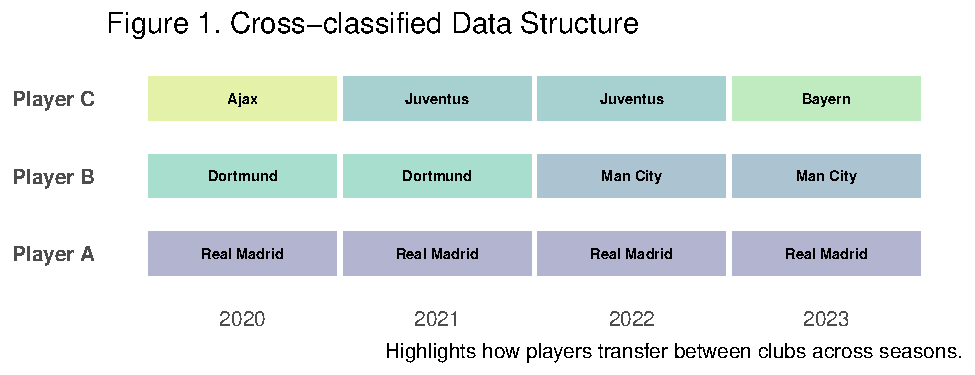
\includegraphics{Project_Paper_12.9_files/figure-pdf/unnamed-chunk-1-1.pdf}

\[
\begin{aligned}
\log(\text{MV})_{tij} = \quad & \gamma_{00} + u_i + v_j \\[6pt]
& + (\gamma_1 + w_{1j})\text{Year}_t + (\gamma_2 + w_{2j})\text{Year}_t^2 + \gamma_3\text{Year}_t^3 \\[6pt]
& + \gamma_4\text{Age}_{ti} + \gamma_5\text{Age}_{ti}^2 \\[6pt]
& + \gamma_6\text{Minutes}_{tij} + \gamma_7\text{Goals}_{tij} + \gamma_8\text{Assists}_{tij} \\[6pt]
& + \gamma_9\text{RedCards}_{tij} + \gamma_{10}\text{YellowCards}_{tij} \\[6pt]
& + \gamma_{11}\text{Foreign}_{tj} + \gamma_{12}\text{UEFA}_{tj} \\[6pt]
& + \beta_1\text{Height}_i + \beta_2\text{Citizen}_{ij} + \boldsymbol{\beta}'_{pos}\mathbf{D}^{pos}_i + \boldsymbol{\beta}'_{reg}\mathbf{D}^{reg}_i \\[6pt]
& + \epsilon_{tij}
\end{aligned}
\]

The model includes three sources of random variation:
\(u_i \sim N(0, \tau^2_u)\) captures persistent player reputation,
\(v_j \sim N(0, \tau^2_v)\) captures baseline club prestige, and
\(\epsilon_{tij} \sim N(0, \sigma^2)\) is the residual. The random
slopes \(w_{1j}\) and \(w_{2j}\) allow clubs to differ in their linear
and quadratic market value trajectories over time; together with
\(v_j\), they follow a multivariate normal distribution with an
unstructured covariance matrix.

Season year is centered at 2020 to isolate the pandemic's structural
impact, with cubic polynomial terms capturing the hypothesized
``Boom-and-Bust'' cycle (see Figure 2). Age is grand-mean centered
(\(\bar{A} = 26.5\) years) with a quadratic term to model the biological
career arc. Minutes played is standardized within each club-year to
measure squad status independent of team rotation policies, while goals
and assists are position-centered to capture performance relative to
role-specific expectations.\footnote{Performance expectations vary by
  role, as a goal from a striker is routine while for a defender is
  exceptional. Position-centering transforms raw counts into
  ``performance above expectation'' metrics, ensuring the model captures
  relative contributions rather than treating goals and assists equally.}
The vectors \(\mathbf{D}^{pos}_i\) and \(\mathbf{D}^{reg}_i\) contain
dummy variables for player position (reference: Attacker) and region of
origin (reference: Europe \& Central Asia), respectively. Citizenship
status (\(\text{Citizen}_{ij}\)) indicates whether player \(i\) holds
citizenship in club \(j\)'s country.

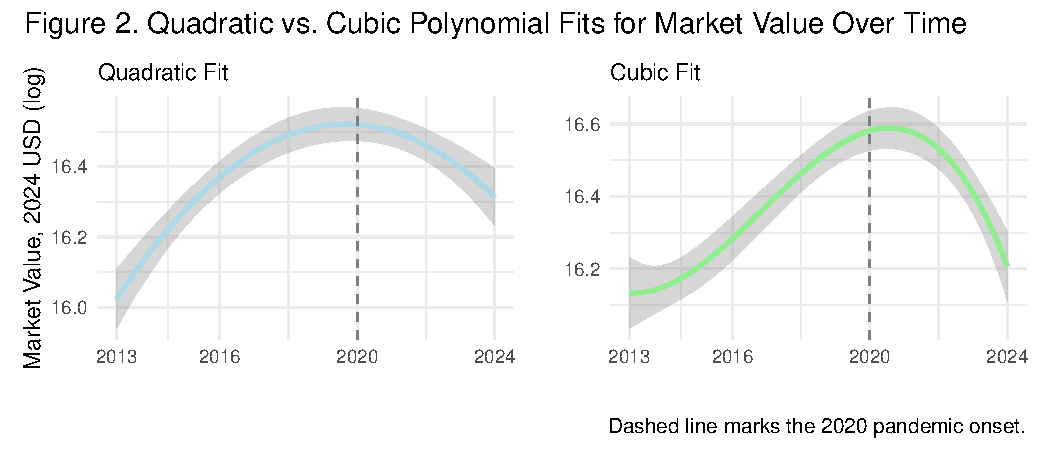
\includegraphics{Project_Paper_12.9_files/figure-pdf/unnamed-chunk-2-1.pdf}

\subsection{Model Testing and Statistical
Software}\label{model-testing-and-statistical-software}

We employed sequential model building: (1) null model for ICC
estimation; (2) linear time polynomial; (3) cubic time polynomial; (4)
random slope for quadratic time at club level\footnote{We excluded
  player-level random slopes due to data sparsity; a majority of players
  appear in the dataset for only one or two seasons, making it
  mathematically impossible to disentangle their individual growth
  trajectories from residual error. In contrast, the club-level data
  provides a robust longitudinal structure with continuous observations
  across the decade, allowing for the stable estimation of club-specific
  market value trajectories.}; (5) player/club-season Level 1 predictors
with quadratic age, and all code is found in Appendix B. Model selection
and comparison was guided by Likelihood Ratio Tests (LRT) to evaluate
the statistical significance of nested model improvements, and the
Akaike Information Criterion (AIC) and Bayesian Information Criterion
(BIC). Models yielding significant LRT results (p\textless.05) and lower
values on both information criteria were retained for subsequent
analysis. We describe each model in Appendix C, Table 1 alongside ICC,
AIC, and BIC values.

All analyses were conducted in R version 4.4.1 using the
\texttt{lme4\ 1.1-37} package for mixed-effects model estimation with a
Restricted Maximum Likelihood (REML) method. REML was selected to
provide unbiased estimates of the variance components by accounting for
the degrees of freedom lost when estimating fixed effects. We utilized
the BOBYQA optimizer, which handles boundary constraints more
effectively than the default Nelder-Mead optimizer, to ensure robust
model convergence given the complexity of the random effects structure.
Significance tests used Satterthwaite approximations via the
\texttt{lmerTest\ 3.1-3} package, as well as our own function to test
random slope variances in Appendix B.

\section{Results}\label{results}

The unconditional means (null) model revealed substantial clustering at
the player level. Player-level variance accounted for 75\% of the total
variance (\(ICC_{player}=.75\)), while club-level variance accounted for
3\% (\(ICC_{club}=.03\)), highlighting that persistent individual
heterogeneity dominates market valuations. Regarding temporal dynamics,
model comparisons favored a cubic fixed effect for season year over a
linear specification, \(\chi^2(2)=45.66, p<.001\). We subsequently
tested for club-specific heterogeneity in growth trajectories. A
likelihood ratio test using a 50:50 mixture of \(\chi^2_1\) and
\(\chi^2_2\) distributions confirmed that adding a random linear slope
significantly improved model fit compared to the random-intercept model,
\(\chi^2(5)=97.13, p<.001\), indicating that clubs differ significantly
not only in their growth rates but also in the curvature of their market
value trajectories. Consequently, our final best-fitting model
incorporates these complex random effects alongside time-varying player
and club predictors (\(\chi^2(19)=5626, p<.001\) compared to random
slopes model). Model comparisons are shown in Appendix C. Our final
model converged successfully with diagnostic plots confirming normality
and homoscedasticity assumptions.

\begin{table}[H]
\centering
\caption{Estimated Variance Components for Final Model}
\centering
\fontsize{11}{13}\selectfont
\begin{tabular}[t]{>{}llrr}
\toprule
Component & Symbol & Variance & SD\\
\midrule
\textbf{Player (Reputation)} & $\tau^2_u$ & 0.9254 & 0.9620\\
\textbf{Club (Baseline Prestige)} & $\tau^2_v$ & 0.0541 & 0.2326\\
\textbf{Club (Linear Growth)} & $\tau^2_{w1}$ & 0.0105 & 0.1025\\
\textbf{Club (Quadratic Curvature)} & $\tau^2_{w2}$ & 0.0073 & 0.0855\\
\textbf{Residual} & $\sigma^2$ & 0.2070 & 0.4550\\
\bottomrule
\end{tabular}
\end{table}

\begin{table}[H]
\centering
\caption{Fixed Effects Estimates from Final Model}
\centering
\resizebox{\ifdim\width>\linewidth\linewidth\else\width\fi}{!}{
\fontsize{10}{12}\selectfont
\begin{threeparttable}
\begin{tabular}[t]{>{}llrrrrl}
\toprule
Predictor & Symbol & $\hat{\gamma}/\hat{\beta}$ & SE & $t$ & \% Change & \\
\midrule
\addlinespace[0.3em]
\multicolumn{7}{l}{\textit{Temporal Dynamics}}\\
\hspace{1em}\textbf{Year (linear)} & $\gamma_1$ & 0.002 & 0.030 & 0.08 & 0.2 & \\
\hspace{1em}\textbf{Year²} & $\gamma_2$ & -0.270 & 0.024 & -11.05 & -23.7 & ***\\
\hspace{1em}\textbf{Year³} & $\gamma_3$ & -0.117 & 0.011 & -10.98 & -11.0 & ***\\
\addlinespace[0.3em]
\multicolumn{7}{l}{\textit{Career Arc}}\\
\hspace{1em}\textbf{Age (linear)} & $\gamma_4$ & 0.019 & 0.004 & 5.02 & 1.9 & ***\\
\hspace{1em}\textbf{Age²} & $\gamma_5$ & -0.024 & 0.000 & -63.08 & -2.4 & ***\\
\addlinespace[0.3em]
\multicolumn{7}{l}{\textit{Performance}}\\
\hspace{1em}\textbf{Goals} & $\gamma_7$ & 0.005 & 0.002 & 2.36 & 0.5 & *\\
\hspace{1em}\textbf{Assists} & $\gamma_8$ & 0.010 & 0.003 & 3.51 & 1.0 & ***\\
\hspace{1em}\textbf{Red cards} & $\gamma_9$ & 0.009 & 0.022 & 0.42 & 0.9 & \\
\hspace{1em}\textbf{Yellow cards} & $\gamma_{10}$ & -0.002 & 0.003 & -0.49 & -0.2 & \\
\hspace{1em}\textbf{Minutes (Z)} & $\gamma_6$ & 0.350 & 0.013 & 26.20 & 41.9 & ***\\
\addlinespace[0.3em]
\multicolumn{7}{l}{\textit{Club Context}}\\
\hspace{1em}\textbf{UEFA Coefficient} & $\gamma_{12}$ & 0.000 & 0.001 & -0.39 & 0.0 & \\
\hspace{1em}\textbf{Foreign players \%} & $\gamma_{11}$ & 0.103 & 0.104 & 0.99 & 10.8 & \\
\addlinespace[0.3em]
\multicolumn{7}{l}{\textit{Player Characteristics}}\\
\hspace{1em}\textbf{Height} & $\beta_1$ & 0.010 & 0.004 & 2.81 & 1.0 & **\\
\hspace{1em}\textbf{Domestic citizen} & $\beta_2$ & -0.185 & 0.031 & -5.89 & -16.9 & ***\\
\addlinespace[0.3em]
\multicolumn{7}{l}{\textit{Position (ref: Attacker)}}\\
\hspace{1em}\textbf{Defender} & $\beta_{pos,1}$ & -0.403 & 0.058 & -6.97 & -33.2 & ***\\
\hspace{1em}\textbf{Goalkeeper} & $\beta_{pos,2}$ & -1.059 & 0.095 & -11.17 & -65.3 & ***\\
\hspace{1em}\textbf{Midfielder} & $\beta_{pos,3}$ & -0.190 & 0.058 & -3.29 & -17.3 & **\\
\addlinespace[0.3em]
\multicolumn{7}{l}{\textit{Region (ref: Europe)}}\\
\hspace{1em}\textbf{East Asia \& Pacific} & $\beta_{reg,1}$ & -0.426 & 0.204 & -2.08 & -34.7 & *\\
\hspace{1em}\textbf{Latin America} & $\beta_{reg,2}$ & 0.188 & 0.061 & 3.09 & 20.7 & **\\
\hspace{1em}\textbf{Middle East \& N. Africa} & $\beta_{reg,3}$ & -0.097 & 0.238 & -0.41 & -9.2 & \\
\hspace{1em}\textbf{North America} & $\beta_{reg,4}$ & -0.059 & 0.217 & -0.27 & -5.7 & \\
\hspace{1em}\textbf{Sub-Saharan Africa} & $\beta_{reg,5}$ & 0.064 & 0.100 & 0.63 & 6.6 & \\
\bottomrule
\end{tabular}
\begin{tablenotes}[para]
\item \textit{Note: } 
\item *** p < .001, ** p < .01, * p < .05
\end{tablenotes}
\end{threeparttable}}
\end{table}

\subsection{Market Evolution}\label{market-evolution}

Using raw polynomials centered at 2020 (\(t=0\)), our model
mathematically pinpoints the moment the market froze. The linear
coefficient at the 2020 baseline is effectively zero
(\(\gamma_1 = 0.00, p = 0.93\)), indicating that at the exact onset of
the pandemic, the relentless inflation of the previous decade came to a
complete halt. The significant negative quadratic (\(\gamma_2 = -0.27\))
and cubic (\(\gamma_3 = -0.12\)) terms confirm the transition from a
pre-2019 ``Boom'' into a structural correction. Figure 3 displays club
specific trajectories, with panels ordered by baseline prestige. Elite
clubs maintain higher valuations throughout, while trajectory curvature
varies substantially. Clubs like Barcelona and Juventus show concave
patterns indicating stagnation, whereas Arsenal and Liverpool display
more resilient recovery and active value generation throughout the
decade.

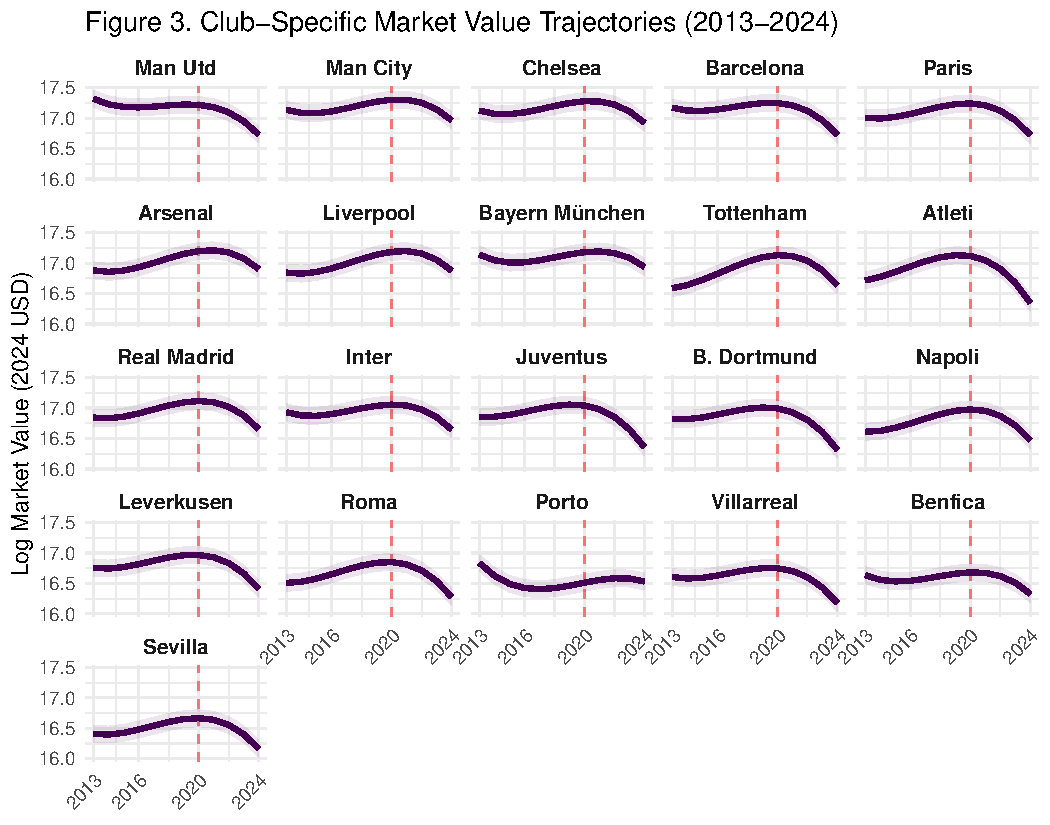
\includegraphics{Project_Paper_12.9_files/figure-pdf/unnamed-chunk-4-1.pdf}

\subsection{Biological Age}\label{biological-age}

Our model predicts the peak age to be 26.9\footnote{We use the delta
  method, specifically Taylor series approximation, to propagate
  uncertainty through nonlinear transformation of
  \(-\gamma_{4} / (2 \times \gamma_{5})\).} for optimal transfer market
value. We visualize in Figure 4 the biological constraints on valuation.
The model predicts peak valuation at age 27, with values dropping
approximately 1.5 log points by age 35, reflecting the market's discount
on older assets with limited resale potential.

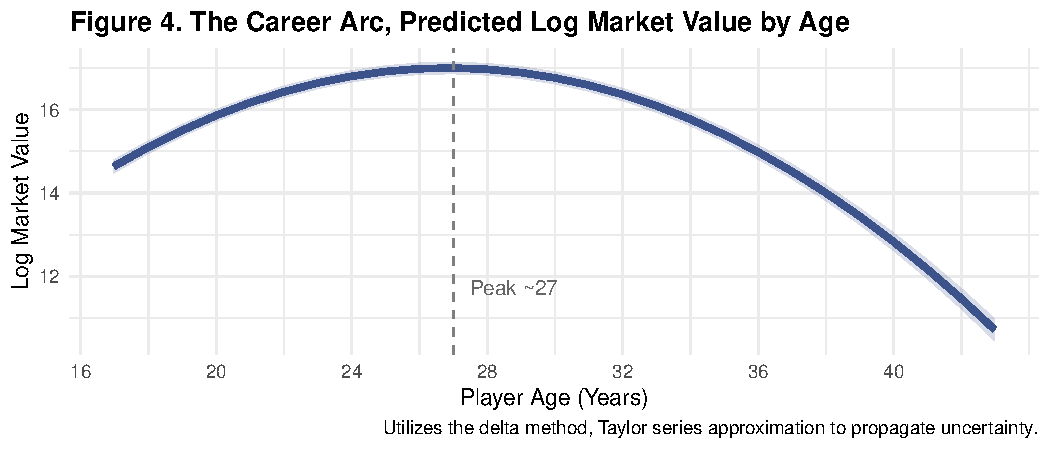
\includegraphics{Project_Paper_12.9_files/figure-pdf/unnamed-chunk-6-1.pdf}

\subsection{\texorpdfstring{\textbf{Contextual Premiums and
Discounts}}{Contextual Premiums and Discounts}}\label{contextual-premiums-and-discounts}

Squad status remains the dominant behavioral driver, with a one standard
deviation increase in relative playing time yielding a 42\% valuation
premium \(\gamma_6=.35\). Homegrown players face a 17\% discount
relative to foreign imports \(\beta_2=-.19\), potentially reflecting the
recruitment premium required to attract international talent. Neither
squad internationalization \(\gamma_{11}=.10, p=.32\) nor UEFA
coefficient (\(p=.70\)) reached significance, suggesting these metrics
add little beyond club random effects. Figure 5 summarizes Level 2 fixed
effects. Attackers command the highest valuations, with Goalkeepers
facing the steepest positional penalty \(\beta_{pos,2}=-1.06\). Among
regions, only Latin America shows a significant premium
\(\beta_{reg, 2}=.19\) suggesting South American players function as a
``premium export brand'' in the global market.

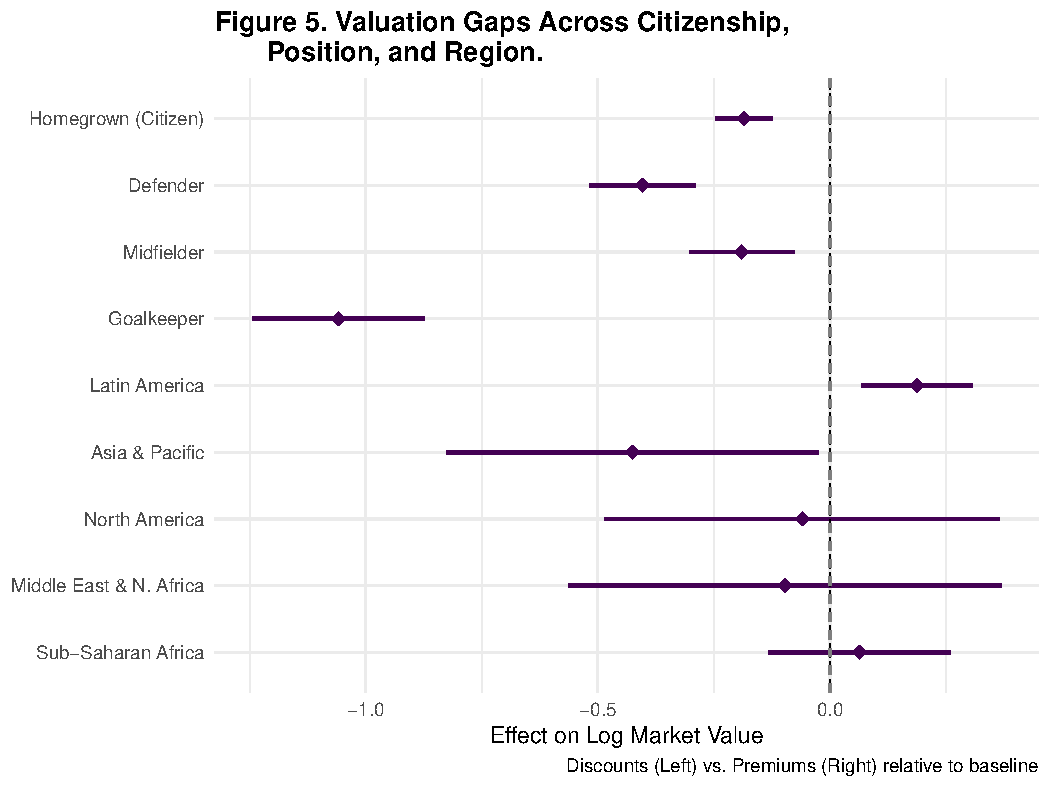
\includegraphics{Project_Paper_12.9_files/figure-pdf/unnamed-chunk-7-1.pdf}

\section{Discussion}\label{discussion}

Our cross-classified multilevel model successfully addressed the
methodological challenge of players transferring between clubs over
time, properly partitioning variance between portable player reputation
and club-level effects. The model converged without warnings, and
diagnostic plots confirmed that distributional assumptions were
reasonably satisfied i.e., player-level random intercepts adhered
closely to normality, while minor tail departures in club-level effects
were expected given only 21 Level 2 units. The residuals versus fitted
values plot showed homoscedastic variance with no systematic patterns,
indicating adequate specification.

The model effectively answered our four research questions. The cubic
time polynomial captured the hypothesized boom-and-bust cycle, with the
2020 centering strategy isolating the pandemic's structural impact. The
quadratic age term confirmed the inverted-U career trajectory,
identifying the peak valuation age. Squad status, operationalized
through within-club standardized minutes, emerged as a stronger
predictor than raw performance metrics, and the inclusion of
region-of-origin effects revealed geographic valuation disparities.

\subsection{Limitations}\label{limitations}

Several limitations warrant consideration. First, our sample comprises
only elite clubs from top European leagues, limiting generalizability to
lower divisions or non-European markets. Second, Transfermarkt
valuations, while validated as proxies for transfer fees, reflect
crowd-sourced estimates rather than actual transaction prices. Third,
our model cannot capture unobserved factors such as injury history,
contract length, or agent influence that likely affect valuations.
Finally, the small number of clubs constrains the complexity of random
effects we could estimate, preventing inclusion of a random cubic slope.

\subsection{Implications}\label{implications}

These findings carry practical implications for European football
economics. Clubs may exploit the domestic discount by investing in
homegrown talent development rather than paying recruitment premiums for
foreign players of comparable quality. The strong signaling value of
playing time suggests that loan strategies to increase minutes for young
players could yield valuation returns beyond skill development alone.
The Latin American premium reflects the continued marketability of South
American talent in European football, potentially driven by historical
success and brand recognition. As the market continues to recover from
pandemic-era corrections, understanding these valuation dynamics becomes
increasingly important for sustainable club financial planning.

\newpage

\section{References}\label{references}

Deloitte. (2021). \emph{Riding the challenge: Annual Review of Football
Finance 2021}. Deloitte Sports Business Group.
\url{https://www2.deloitte.com/uk/en/pages/sports-business-group/articles/annual-review-of-football-finance-europe.html}

Deloitte. (2024). Annual review of football finance 2024: European
football market revenue.
\url{https://www.deloitte.com/uk/en/about/press-room/deloitte-annual-review-of-football-finance-european-football-market-revenue.html}

Drewes, M., Daumann, F., \& Follert, F. (2021). Exploring the sports
economic impact of COVID-19 on professional soccer. \emph{Soccer \&
Society, 22}(1-2), 125-137.
\url{https://doi.org/10.1080/14660970.2020.1802256}

Herm, S., Callsen-Bracker, H. M., \& Kreis, H. (2014). When the crowd
evaluates soccer players' market values: Accuracy and evaluation
attributes of an online community. \emph{Sport Management Review,
17}(4), 484-492. \url{https://doi.org/10.1016/j.smr.2013.12.006}

Maas, C. J. M., \& Hox, J. J. (2004). Robustness issues in multilevel
regression analysis. \emph{Statistica Neerlandica, 58}(2), 127-137.
\url{https://doi.org/10.1046/j.0039-0402.2003.00252.x}

Poli, R., Ravenel, L., \& Besson, R. (2017). \emph{Transfer market
analysis} (CIES Football Observatory Monthly Report No.~27). CIES
Football Observatory.
\url{https://football-observatory.com/IMG/sites/mr/mr27/en/}

\clearpage

\newpage

\section{Appendix A}\label{appendix-a}

\subsection*{\texorpdfstring{Table 1: Variable Descriptions and
Descriptive Statistics
(\emph{N}=7,168)}{Table 1: Variable Descriptions and Descriptive Statistics (N=7,168)}}\label{table-1-variable-descriptions-and-descriptive-statistics-n7168}
\addcontentsline{toc}{subsection}{Table 1: Variable Descriptions and
Descriptive Statistics (\emph{N}=7,168)}

\begin{table}[!h]
\centering\begingroup\fontsize{10}{12}\selectfont

\resizebox{\ifdim\width>\linewidth\linewidth\else\width\fi}{!}{
\begin{tabular}{>{\raggedright\arraybackslash}p{5cm}>{\raggedright\arraybackslash}p{4cm}>{\raggedright\arraybackslash}p{5cm}}
\toprule
Description & Raw Stats (Mean/SD) & Transformation Strategy\\
\midrule
\addlinespace[0.3em]
\multicolumn{3}{l}{\textbf{Continuous Variables}}\\
\hspace{1em}\textbf{Market Value (2024 USD)} & \$25.8M (29.0M) & \em{Log-transformed (ln)}\\
\hspace{1em}\textbf{Season Year} & 2018.63 (3.47) & \em{Centered at 2020 (0 = 2020)}\\
\hspace{1em}\textbf{Player Age (Years)} & 26.50 (4.58) & \em{Grand-mean centered + Quadratic}\\
\hspace{1em}\textbf{Height (cm)} & 182.10 (6.84) & \em{Grand-mean centered}\\
\hspace{1em}\textbf{Minutes Played} & 1761.77 (1337.70) & \em{Z-scored within Club-Year}\\
\hspace{1em}\textbf{Goals Scored} & 3.41 (6.25) & \em{Centered by Position Mean}\\
\hspace{1em}\textbf{Assists Made} & 2.79 (4.00) & \em{Centered by Position Mean}\\
\hspace{1em}\textbf{Club Foreign \%} & 63.5\% (11.1\%) & \em{Grand-mean centered}\\
\hspace{1em}\textbf{UEFA Coefficient} & 20.42 (6.89) & \em{Year-mean centered}\\
\hspace{1em}\textbf{Red Cards} & 0.07 (0.28) & \em{Raw count}\\
\hspace{1em}\textbf{Yellow Cards} & 3.42 (3.60) & \em{Raw count}\\
\addlinespace[0.3em]
\multicolumn{3}{l}{\textbf{Categorical Variables}}\\
\hspace{1em}\textbf{Citizenship (Homegrown)} &  & \em{Binary (1=Citizen)}\\
\hspace{1em}\textbf{- No} & 4498 (62.8\%) & \em{}\\
\hspace{1em}\textbf{- Yes} & 2567 (35.8\%) & \em{}\\
\hspace{1em}\textbf{- NA} & 103 (1.4\%) & \em{}\\
\hspace{1em}\textbf{Primary Position} &  & \em{Factor (Ref: Attack)}\\
\hspace{1em}\textbf{- Attack} & 1925 (26.9\%) & \em{}\\
\hspace{1em}\textbf{- Defender} & 2448 (34.2\%) & \em{}\\
\hspace{1em}\textbf{- Goalkeeper} & 605 (8.4\%) & \em{}\\
\hspace{1em}\textbf{- Midfield} & 2190 (30.6\%) & \em{}\\
\hspace{1em}\textbf{Region of Origin} &  & \em{Factor (Ref: Europe)}\\
\hspace{1em}\textbf{- East Asia \& Pacific} & 69 (1.0\%) & \em{}\\
\hspace{1em}\textbf{- Europe \& Central Asia} & 5139 (71.7\%) & \em{}\\
\hspace{1em}\textbf{- Latin America \& Caribbean} & 1441 (20.1\%) & \em{}\\
\hspace{1em}\textbf{- Middle East \& North Africa} & 56 (0.8\%) & \em{}\\
\hspace{1em}\textbf{- North America} & 52 (0.7\%) & \em{}\\
\hspace{1em}\textbf{- Sub-Saharan Africa} & 303 (4.2\%) & \em{}\\
\hspace{1em}\textbf{- NA} & 108 (1.5\%) & \em{}\\
\bottomrule
\end{tabular}}
\endgroup{}
\end{table}

\newpage

\section{Appendix B}\label{appendix-b}

\subsection{Annotated Model Syntax}\label{annotated-model-syntax}

\small

\begin{Shaded}
\begin{Highlighting}[]
\FunctionTok{library}\NormalTok{(lme4)}
\FunctionTok{library}\NormalTok{(lmerTest)}

\CommentTok{\# Model control for convergence}
\NormalTok{strict\_control }\OtherTok{\textless{}{-}} \FunctionTok{lmerControl}\NormalTok{(}\AttributeTok{optimizer =} \StringTok{"bobyqa"}\NormalTok{)}

\CommentTok{\#\_\_\_\_\_\_\_\_\_\_\_\_\_\_\_\_\_\_\_\_\_\_\_\_\_\_\_\_\_\_\_\_\_\_\_\_\_\_\_\_\_\_\_\_\_\_\_\_\_\_\_\_\_\_\_\_\_\_\_\_\_\_\_\_\_\_\_\_\_\_\_\_\_\_\_\_\_\_}
\CommentTok{\# MODEL SPECIFICATION \& FITTING}

\CommentTok{\# 1. MODEL NULL (Unconditional Means)}
\CommentTok{\# Purpose: Partition variance (calculate ICC) between Player and Club levels}
\NormalTok{model\_null }\OtherTok{\textless{}{-}} \FunctionTok{lmer}\NormalTok{(usd\_revenue\_2024\_log }\SpecialCharTok{\textasciitilde{}}\NormalTok{ (}\DecValTok{1}\SpecialCharTok{|}\NormalTok{player\_id) }\SpecialCharTok{+}\NormalTok{ (}\DecValTok{1}\SpecialCharTok{|}\NormalTok{club\_id), }
                   \CommentTok{\# the following repeats for all models captured as "..."}
                   \AttributeTok{data =}\NormalTok{ clean\_player\_df, }
                   \AttributeTok{REML =} \ConstantTok{TRUE}\NormalTok{, }
                   \AttributeTok{control =}\NormalTok{ strict\_control)}

\CommentTok{\# 2. MODEL LINEAR TIME TREND}
\CommentTok{\# Purpose: Test for general linear inflation in market values }
\DocumentationTok{\#\# (Base model for time)}
\NormalTok{model\_time\_linear }\OtherTok{\textless{}{-}} \FunctionTok{lmer}\NormalTok{(usd\_revenue\_2024\_log }\SpecialCharTok{\textasciitilde{}}\NormalTok{ season\_year\_c }\SpecialCharTok{+} 
\NormalTok{                          (}\DecValTok{1}\SpecialCharTok{|}\NormalTok{player\_id) }\SpecialCharTok{+}\NormalTok{ (}\DecValTok{1}\SpecialCharTok{|}\NormalTok{club\_id), ...) }\CommentTok{\# Random Effects}

\CommentTok{\# 3. MODEL CUBIC TIME TREND (Fixed Effects)}
\CommentTok{\# Purpose: Test for non{-}linear "Boom and Bust" cycles}
\NormalTok{model\_time\_cubic }\OtherTok{\textless{}{-}} \FunctionTok{lmer}\NormalTok{(usd\_revenue\_2024\_log }\SpecialCharTok{\textasciitilde{}} 
                           \CommentTok{\# Temporal Controls}
                           \DocumentationTok{\#\# (raw=TRUE for interpretability)}
                           \FunctionTok{poly}\NormalTok{(season\_year\_c, }\DecValTok{3}\NormalTok{, }\AttributeTok{raw=}\ConstantTok{TRUE}\NormalTok{) }\SpecialCharTok{+} 
\NormalTok{                         (}\DecValTok{1}\SpecialCharTok{|}\NormalTok{player\_id) }\SpecialCharTok{+}\NormalTok{ (}\DecValTok{1}\SpecialCharTok{|}\NormalTok{club\_id), ...)}

\CommentTok{\# 4. MODEL RANDOM QUADRATIC SLOPE (Club Level)}
\CommentTok{\# Purpose: Test if trajectory curvature varies by club }
\DocumentationTok{\#\# (Linear slope model omitted for brevity)}
\NormalTok{model\_slope\_quadratic }\OtherTok{\textless{}{-}} \FunctionTok{lmer}\NormalTok{(usd\_revenue\_2024\_log }\SpecialCharTok{\textasciitilde{}} 
                                \FunctionTok{poly}\NormalTok{(season\_year\_c, }\DecValTok{3}\NormalTok{, }\AttributeTok{raw=}\ConstantTok{TRUE}\NormalTok{) }\SpecialCharTok{+} 
\NormalTok{                                (}\DecValTok{1}\SpecialCharTok{|}\NormalTok{player\_id) }\SpecialCharTok{+} 
\NormalTok{                                (}\FunctionTok{poly}\NormalTok{(season\_year\_c, }\DecValTok{2}\NormalTok{, }\AttributeTok{raw=}\ConstantTok{TRUE}\NormalTok{) }\SpecialCharTok{|}\NormalTok{ club\_id), }
\NormalTok{                              ...)}

\CommentTok{\# 5. MODEL (FINAL): FULL SPECIFICATION}
\CommentTok{\# Purpose: Estimate marginal effects of performance, status, }
\DocumentationTok{\#\# and context controlling for time}
\NormalTok{model\_player }\OtherTok{\textless{}{-}} \FunctionTok{lmer}\NormalTok{(}
\NormalTok{  usd\_revenue\_2024\_log }\SpecialCharTok{\textasciitilde{}} 
    \FunctionTok{poly}\NormalTok{(season\_year\_c, }\DecValTok{3}\NormalTok{, }\AttributeTok{raw=}\ConstantTok{TRUE}\NormalTok{) }\SpecialCharTok{+}          
    \FunctionTok{poly}\NormalTok{(age\_c, }\DecValTok{2}\NormalTok{, }\AttributeTok{raw=}\ConstantTok{TRUE}\NormalTok{) }\SpecialCharTok{+}                  \CommentTok{\# Career Arc}
    \CommentTok{\# Player context}
\NormalTok{    height\_c }\SpecialCharTok{+}\NormalTok{ position }\SpecialCharTok{+}\NormalTok{ Region }\SpecialCharTok{+}\NormalTok{ citizen\_of\_club\_country }\SpecialCharTok{+} 
    \CommentTok{\# Performance}
\NormalTok{    goals }\SpecialCharTok{+}\NormalTok{ assists }\SpecialCharTok{+}\NormalTok{ red\_cards }\SpecialCharTok{+}\NormalTok{ yellow\_cards }\SpecialCharTok{+}\NormalTok{ minutes\_played }\SpecialCharTok{+} 
\NormalTok{    uefa\_coefficient }\SpecialCharTok{+}\NormalTok{ foreign\_players }\SpecialCharTok{+}        \CommentTok{\# club fixed effects}
\NormalTok{    (}\DecValTok{1}\SpecialCharTok{|}\NormalTok{player\_id) }\SpecialCharTok{+}\NormalTok{ (}\FunctionTok{poly}\NormalTok{(season\_year\_c, }\DecValTok{2}\NormalTok{, }\AttributeTok{raw=}\ConstantTok{TRUE}\NormalTok{) }\SpecialCharTok{|}\NormalTok{ club\_id), }
\NormalTok{    ...)}

\CommentTok{\#\_\_\_\_\_\_\_\_\_\_\_\_\_\_\_\_\_\_\_\_\_\_\_\_\_\_\_\_\_\_\_\_\_\_\_\_\_\_\_\_\_\_\_\_\_\_\_\_\_\_\_\_\_\_\_\_\_\_\_\_\_\_\_\_\_\_\_\_\_\_\_\_\_\_\_\_\_\_}
\CommentTok{\# LIKELIHOOD RATIO }\AlertTok{TEST}\CommentTok{ (MIXTURE DISTRIBUTION)}

\CommentTok{\# LRT test for 2 random slopes}
\NormalTok{calculate\_lrt\_mixture }\OtherTok{\textless{}{-}} \ControlFlowTok{function}\NormalTok{(reduced\_model, full\_model) \{}
  
  \CommentTok{\# 1. Extract Log{-}Likelihoods}
\NormalTok{  ll\_reduced }\OtherTok{=} \FunctionTok{as.numeric}\NormalTok{(}\FunctionTok{logLik}\NormalTok{(reduced\_model))}
\NormalTok{  ll\_full }\OtherTok{=} \FunctionTok{as.numeric}\NormalTok{(}\FunctionTok{logLik}\NormalTok{(full\_model))}
  
  \CommentTok{\# 2. Calculate LRT Statistic}
\NormalTok{  lrt\_stat }\OtherTok{=} \SpecialCharTok{{-}}\DecValTok{2} \SpecialCharTok{*}\NormalTok{ (ll\_reduced }\SpecialCharTok{{-}}\NormalTok{ ll\_full)}
  
  \CommentTok{\# 3. Calculate Difference in Parameters (df)}
\NormalTok{  df\_reduced }\OtherTok{=} \FunctionTok{attr}\NormalTok{(}\FunctionTok{logLik}\NormalTok{(reduced\_model), }\StringTok{"df"}\NormalTok{)}
\NormalTok{  df\_full }\OtherTok{=} \FunctionTok{attr}\NormalTok{(}\FunctionTok{logLik}\NormalTok{(full\_model), }\StringTok{"df"}\NormalTok{)}
\NormalTok{  df\_diff }\OtherTok{=}\NormalTok{ df\_full }\SpecialCharTok{{-}}\NormalTok{ df\_reduced}
  
  \CommentTok{\# 4. Calculate P{-}Value based on the difference}
  
  \ControlFlowTok{if}\NormalTok{ (df\_diff }\SpecialCharTok{==} \DecValTok{3}\NormalTok{) \{}
    \CommentTok{\# Going from 2 Random Effects (Int+Lin) {-}\textgreater{} 3 Random Effects Int+Lin+Quad}
    \CommentTok{\# We add 1 variance + 2 covariances = 3 parameters.}
    \CommentTok{\# The mixture is 0.5 * ChiSq(2) + 0.5 * ChiSq(3)}
\NormalTok{    p\_val }\OtherTok{=} \FloatTok{0.5} \SpecialCharTok{*} \FunctionTok{pchisq}\NormalTok{(lrt\_stat, }\AttributeTok{df =} \DecValTok{2}\NormalTok{, }\AttributeTok{lower.tail =} \ConstantTok{FALSE}\NormalTok{) }\SpecialCharTok{+} 
      \FloatTok{0.5} \SpecialCharTok{*} \FunctionTok{pchisq}\NormalTok{(lrt\_stat, }\AttributeTok{df =} \DecValTok{3}\NormalTok{, }\AttributeTok{lower.tail =} \ConstantTok{FALSE}\NormalTok{)}
\NormalTok{    \} }\ControlFlowTok{else} \ControlFlowTok{if}\NormalTok{ (df\_diff }\SpecialCharTok{==} \DecValTok{2}\NormalTok{) \{}
    \CommentTok{\# Going from 1 Random Effect (Int) {-}\textgreater{} 2 Random Effects (Int+Lin)}
    \CommentTok{\# Adds 1 variance + 1 covariance = 2 parameters}
\NormalTok{    p\_val }\OtherTok{=} \FloatTok{0.5} \SpecialCharTok{*} \FunctionTok{pchisq}\NormalTok{(lrt\_stat, }\AttributeTok{df =} \DecValTok{1}\NormalTok{, }\AttributeTok{lower.tail =} \ConstantTok{FALSE}\NormalTok{) }\SpecialCharTok{+} 
      \FloatTok{0.5} \SpecialCharTok{*} \FunctionTok{pchisq}\NormalTok{(lrt\_stat, }\AttributeTok{df =} \DecValTok{2}\NormalTok{, }\AttributeTok{lower.tail =} \ConstantTok{FALSE}\NormalTok{)}
\NormalTok{    \} }\ControlFlowTok{else} \ControlFlowTok{if}\NormalTok{ (df\_diff }\SpecialCharTok{==} \DecValTok{1}\NormalTok{) \{}
    \CommentTok{\# Adding a single parameter (e.g. just a variance, no covariance)}
\NormalTok{    p\_val }\OtherTok{=} \FloatTok{0.5} \SpecialCharTok{*} \FunctionTok{pchisq}\NormalTok{(lrt\_stat, }\AttributeTok{df =} \DecValTok{0}\NormalTok{, }\AttributeTok{lower.tail =} \ConstantTok{FALSE}\NormalTok{) }\SpecialCharTok{+} 
      \FloatTok{0.5} \SpecialCharTok{*} \FunctionTok{pchisq}\NormalTok{(lrt\_stat, }\AttributeTok{df =} \DecValTok{1}\NormalTok{, }\AttributeTok{lower.tail =} \ConstantTok{FALSE}\NormalTok{)}
\NormalTok{    \} }\ControlFlowTok{else}\NormalTok{ \{}
    \CommentTok{\# Fallback for standard fixed effects comparisons}
\NormalTok{    p\_val }\OtherTok{=} \FunctionTok{pchisq}\NormalTok{(lrt\_stat, }\AttributeTok{df =}\NormalTok{ df\_diff, }\AttributeTok{lower.tail =} \ConstantTok{FALSE}\NormalTok{)\}}
  
  \CommentTok{\# Output}
  \FunctionTok{cat}\NormalTok{(}\StringTok{"LRT Statistic:"}\NormalTok{, }\FunctionTok{round}\NormalTok{(lrt\_stat, }\DecValTok{4}\NormalTok{),  df\_diff, }\StringTok{"}\SpecialCharTok{\textbackslash{}n}\StringTok{"}\NormalTok{)}
  \FunctionTok{cat}\NormalTok{(}\StringTok{"P{-}Value:       "}\NormalTok{, }\FunctionTok{format.pval}\NormalTok{(p\_val, }\AttributeTok{eps =}\NormalTok{ .}\DecValTok{0001}\NormalTok{), }\StringTok{"}\SpecialCharTok{\textbackslash{}n}\StringTok{"}\NormalTok{)\}}
\end{Highlighting}
\end{Shaded}

We test whether a random slope with quadratic season year at the club
level has better fit to the data. We find evidence supporting the need
to include these random slopes using a likelihood ratio test with an
alternative hypothesis, \(H_A=\tau_{11} > 0\) since variance should be
larger than 0. To test this hypothesis we use the likelihood ratio test
(LRT) simply by
\(-2[\text{log likelihood}_{reduced} - \text{log likelihood}_{full}]\)
to examine the difference.

\begin{verbatim}
LRT Statistic: 97.1306 
Parameter Diff: 5 
Distribution:   Standard ChiSq(5) 
P-Value:        < 0.0001 
\end{verbatim}

\newpage

\normalsize

\section{Appendix C}\label{appendix-c}

\subsection*{Table 1. Model Fit Comparison (AIC, BIC, and
ICC)}\label{table-1.-model-fit-comparison-aic-bic-and-icc}
\addcontentsline{toc}{subsection}{Table 1. Model Fit Comparison (AIC,
BIC, and ICC)}

\begin{longtable}[]{@{}
  >{\raggedright\arraybackslash}p{(\columnwidth - 8\tabcolsep) * \real{0.2055}}
  >{\raggedright\arraybackslash}p{(\columnwidth - 8\tabcolsep) * \real{0.3425}}
  >{\raggedright\arraybackslash}p{(\columnwidth - 8\tabcolsep) * \real{0.1781}}
  >{\raggedright\arraybackslash}p{(\columnwidth - 8\tabcolsep) * \real{0.1370}}
  >{\raggedright\arraybackslash}p{(\columnwidth - 8\tabcolsep) * \real{0.1370}}@{}}
\toprule\noalign{}
\endhead
\bottomrule\noalign{}
\endlastfoot
\textbf{Models} & \textbf{Purpose \& Research Justification} &
ICCplayer/ club & AIC & BIC \\
\textbf{Null} & Calculate ICC and partition variance between players and
clubs before adding predictors & .75/.03 & 20105.19 & 20132.62 \\
\textbf{Time Linear} & Test for a general linear trend in market value
growth & .76/.03 & 20050.17 & 20084.46 \\
\textbf{Time Cubic} & Test for non-linear market dynamics (e.g.,
acceleration or deceleration/plateaus) & .76/.03 & 20021.61 &
20069.61 \\
\textbf{Random Slope Quadratic} & Test if the growth curvature varies by
club & .76/.04 & 19934.48 & 20016.76 \\
\textbf{Varying Level 1 fixed effects} & Estimate the marginal value of
performance metrics and player/club characteristics controlling for time
& .78/.05 & 14467.31 & 14679.87 \\
\textbf{Final Model Selection} & Compare models using LRT, AIC/BIC, and
residual diagnostics (QQ plots) to select the most parsimonious and
robust fit & & & \\
\end{longtable}

\newpage

\subsection*{}\label{section}
\addcontentsline{toc}{subsection}{}

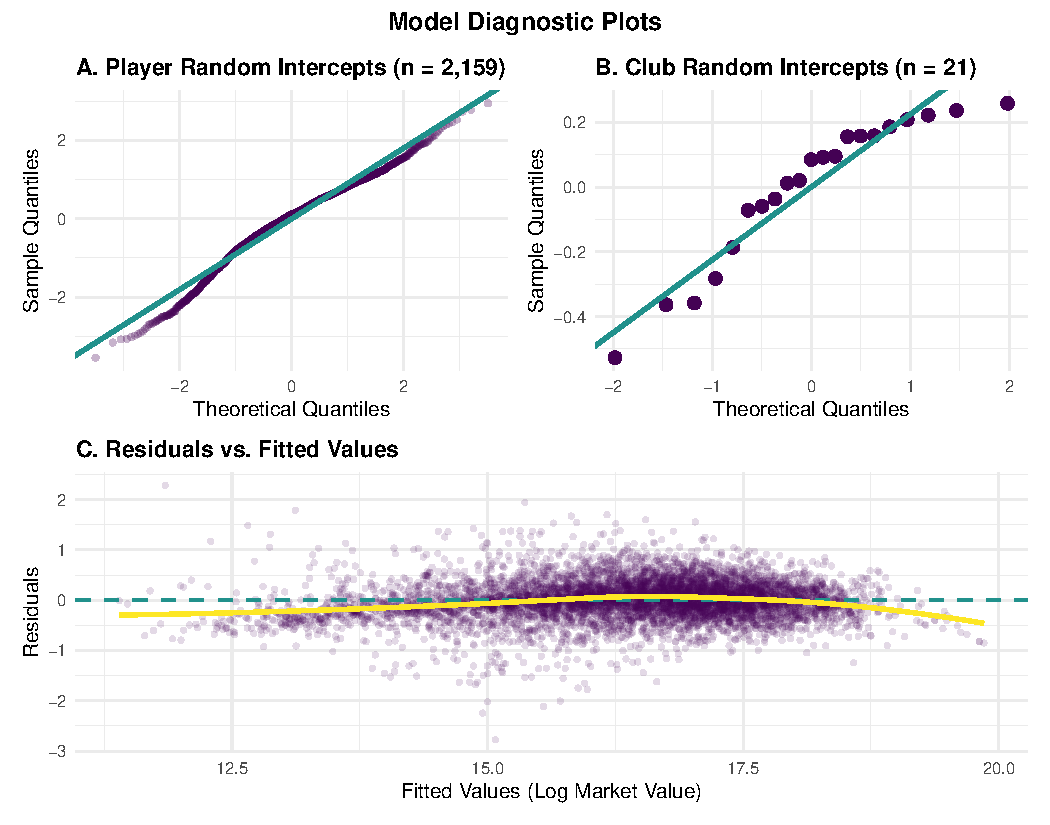
\includegraphics{Project_Paper_12.9_files/figure-pdf/unnamed-chunk-11-1.pdf}

Q-Q plots confirmed that player-level random intercepts (n = 2,159)
adhered well to normality, while club-level random effects (n = 21)
showed minor tail departures expected with few Level 2 units (Maas \&
Hox, 2004). The residuals versus fitted values plot revealed
homoscedastic variance with no systematic patterns.

\newpage

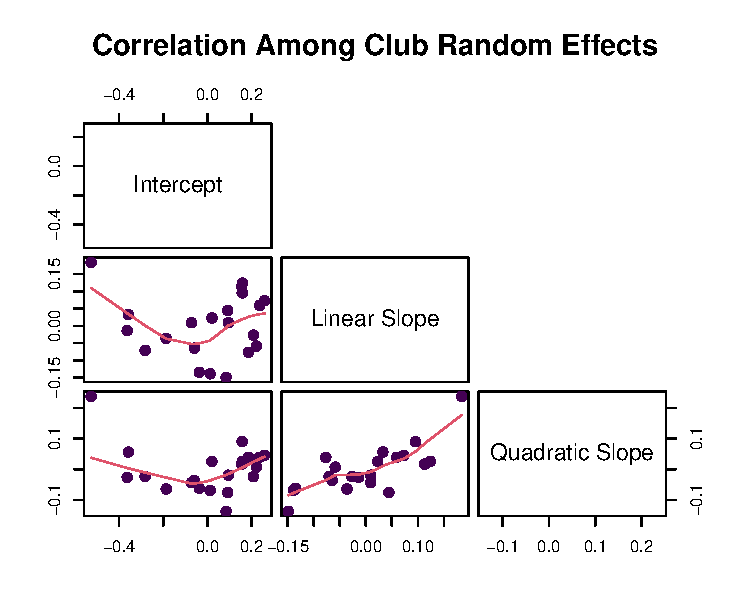
\includegraphics{Project_Paper_12.9_files/figure-pdf/unnamed-chunk-12-1.pdf}

HEAD The correlation between club intercept and linear slope was weak
and non-significant (r = -0.06), suggesting minimal
regression-to-the-mean. The positive correlation between linear and
quadratic slopes (r = 0.75) indicates that clubs with faster initial
growth experienced more pronounced curvature around the pandemic period.

\newpage

\section{Appendix D}\label{appendix-d}

\subsection*{Acknowledgement of AI
Assistance}\label{acknowledgement-of-ai-assistance}
\addcontentsline{toc}{subsection}{Acknowledgement of AI Assistance}

We acknowledge the use of AI-assisted tools (GitHub Copilot and Claude)
during the preparation of this manuscript. These tools were used for:

\begin{enumerate}
\def\labelenumi{\arabic{enumi}.}
\item
  \textbf{Coding assistance}: Generating and debugging R code for data
  visualization, particularly for creating the faceted club trajectory
  plots (Figure 3) and diagnostic visualizations.
\item
  \textbf{Resolving convergence issues}: Troubleshooting model
  convergence problems with the cross-classified multilevel model,
  including optimizer selection (BOBYQA) and parameter constraints.
\item
  \textbf{Code documentation}: Improving comments and annotations in the
  model syntax presented in Appendix B.
\end{enumerate}

All statistical analyses, interpretations, and substantive conclusions
were developed and verified by the authors. The AI tools served as
coding assistants and did not contribute to the research design, data
collection, or theoretical framework of this study.




\end{document}
